\chapter{Implémentation}
        \section{Choix des technologies}
        Au cours de la réalisation d'un logiciel numérique,
        l'une des étapes les plus importantes est de choisir la bonne pile technologique. 
        Pourquoi? Parce qu'il s'agit de créer un produit qui ne consiste pas uniquement
        à concevoir une interface utilisateur agréable et une expérience utilisateur 
        pratique; il s'agit également de concevoir un produit stable, sécurisé et 
        maintenable qui, non seulement est en mesure de charmer les utilisateurs mais encore, vous 
        permettra de faire évoluer l'entreprise.
        \paragraph{}
        Chaque couche de l'application est construite au-dessus d'une autre, 
        formant une pile. Cela rend les technologies Web fortement dépendantes 
        les unes des autres. L'image \ref{fig:pile} montre les principaux éléments constitutifs 
        d'une pile technologique typique; cependant, il peut y avoir d'autres éléments de 
        soutien impliqués.
        \begin{figure}[t]
                \centering
                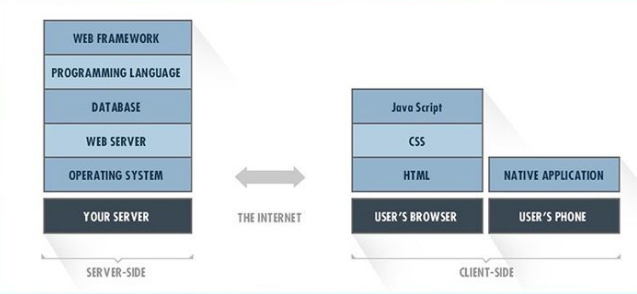
\includegraphics[scale=0.5]{images/Implementation/pile.png}
                \caption{Modèle du cycle de vie en cascade \cite{Bulatovych}}
                \label{fig:pile}
        \end{figure}
        \subsection{Frontend}
        L'interface utilisateur est également appelée côté client, car les utilisateurs voient et interagissent 
        avec cette partie d'une application. Pour une application web, cette interaction s'effectue 
        dans un navigateur web et est possible grâce à de nombreux outils de programmation (Tableau \ref{tab:techoFrontend}). 
        Les applications Web destinées aux clients sont généralement créées à l'aide d'une combinaison 
        de JavaScript, HTML et CSS.
        \paragraph{Outils que nous utilisons pour le développement frontend:}
        \paragraph{HTML: }
        (Hypertext Markup Language) est un langage de programmation utilisé pour décrire 
        la structure des informations présentées sur une page Web. 
        \textit{Le World Wide Web est aujourd'hui l'une des sources d'information les plus 
        importantes. La plupart des données sur le Web sont disponibles sous forme de 
        pages encodées dans des langages de balisage tels que HTML destinés aux 
        navigateurs visuels \cite{yang2003html}.} 
        \par 
        Pour la réalisation de GeoTechMap, nou utilisons HTML5 qui est la cinquième et dernière 
        édition recommandée par le World Wide Web Consortium (W3C) \cite{brooks2010world}.
        \paragraph{CSS: }
         (Cascading Style Sheets) est un langage de feuille de style qui décrit 
        l'apparence et la mise en forme d'un document écrit en HTML. CSS est utilisé 
        pour annoter du texte et incorporer des balises dans des documents électroniques stylisés.
        Le CSS est encore plus important car il doit être pris en compte pour rendre l'applicatgion responsive.
        L'interface utilisateur doit pouvoir s'adapter à n'importe quelle dimention d'écran 
        d'autant plus que nous constatons la montée du trafic web via les téléphones mobiles (Figure \ref{fig:statMobile}).
        \begin{figure}[t]
                \centering
                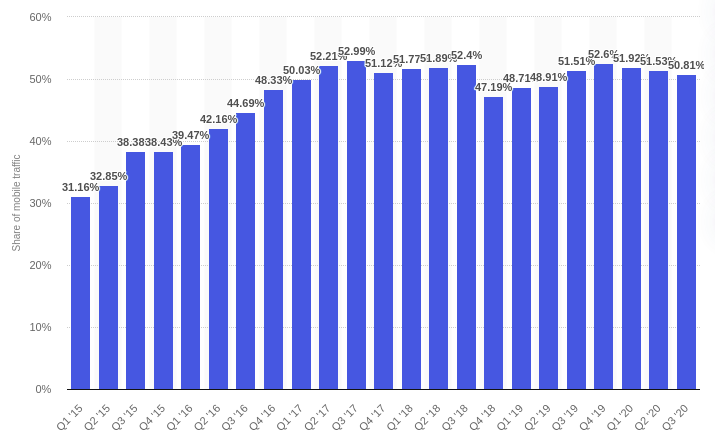
\includegraphics[scale=0.5]{images/Implementation/statMobile.png}
                \caption{
                        Pourcentage du trafic du site Web sur les appareils 
                        mobiles dans le monde du 1er trimestre 2015 au 3ème trimestre 2020 \cite{linkstatmobile}}
                \label{fig:statMobile}
        \end{figure}
        \paragraph{JavaScript (ou JS): }
         C'est la troisième technologie principale pour créer 
        l'interface d'une application Web. JavaScript est couramment utilisé pour créer des 
        pages Web dynamiques et interactives. En d'autres termes, il permet des animations 
        Web simples et complexes, qui contribuent grandement à une expérience utilisateur 
        positive.
        \par
        \textit{JavaScript est devenu le langage de facto pour la programmation Web côté client \cite{gardner2012towards}.}
        \paragraph{React: }
        C'est une bibliothèque JavaScript pour créer des interfaces utilisateur.
        ReactJS offre des solutions élégantes à certains des problèmes les plus 
        persistants de la programmation frontend, vous permettant de créer facilement 
        des applications Web dynamiques et interactives. Il est rapide, évolutif, flexible, 
        puissant et dispose d’une solide communauté de développeurs qui se développe 
        rapidement. \textit{Il s'agit actuellement de la bibliothèque JS frontale la plus populaire \cite{aggarwal2018modern}.}  
        \par    
        \begin{table}
                \centering
                \begin{tabular}{|p{0.30\linewidth}|p{0.10\linewidth}|p{0.60\linewidth}|}
                \hline
                        \textbf{Technologie}&\textbf{Version}&\textbf{Détails}\\
                        \hline
                        HTML&
                        5&
                        HTML5 est conçu pour rendre le développement de ces applications Web 
                        riches plus facile, plus naturel et plus logique, où les développeurs 
                        peuvent concevoir et créer une seule fois, et les déployer n'importe où. 
                        HTML5 rend également les applications Web plus utilisables, car il supprime 
                        le besoin de plugins \cite{wang2013definitive}.
                        \\
                        \hline
                        CSS&
                        3&
                        bla
                        \\
                        \hline
                        JS&
                        ES6&
                        « ES » est l’abréviation d’ECMAScript, le standard sur lequel repose JavaScript.
                        Tous les navigateurs modernes supportent l’ES6 depuis un moment, et les 
                        frameworks majeurs (Angular, React, Vue…) utilisent tous cette nouvelle version de JavaScript
                        \\
                        \hline
                        React&
                        17&
                        \textit{Bien que React v17 ne propose aucune nouvelle fonctionnalité, 
                        il établit une base solide pour les versions à venir en abordant directement 
                        l'expérience de mise à niveau et en alignant plus étroitement le comportement 
                        de React sur les navigateurs modernes \cite{Vardhan2020}.}
                        \\
                        \hline
                      
                \end{tabular}
                \caption{Les technologies utilisées pour le développement du frontend de GeoTechMap} 
                \label{tab:techoFrontend}
        \end{table}
        \par
        \subsection{Backend}
        Le backend, qui n'est pas visible pour les utilisateurs finaux, implique la logique métier, 
        l'authentification, la gestion de la base de données et les synchronisations avec 
        l'application cliente. Également appelé côté serveur, il est composé d'un serveur, d'une base 
        de données et d'applications qui s'exécutent dessus.
        \par 
        Même si le backend fonctionne en dehors de la scène et n'est pas visible pour les utilisateurs, 
        c'est le moteur qui pilote votre application et met en œuvre sa logique. Le serveur Web, qui 
        fait partie du backend, accepte les requêtes d'un navigateur, traite ces requêtes selon une 
        certaine logique, se tourne vers la base de données si nécessaire et renvoie le contenu pertinent. 
        \par 
        \textit{Les applications Web sophistiquées d'aujourd'hui ne peuvent pas fonctionner sans
         les services frontaux et backend \cite{abdullah2014frontend}.}

        \subsubsection{Système d'exploitation}
        Le système d'exploitation installé sur le serveur est le plus souvent Windows ou Linux.
        Dans notre cas, il s'agit de Linux pour plusieurs raisons.
        \textit{Les systèmes Linux ont tendance à être plus dynamiques que les 
        systèmes Windows, en raison du taux rapide de mises à jour  
        dans de nombreux projets Linux \cite{ovadia2014linux}.}
        \par
        En effet, la liste des avantages de Linux 
        est longue. Citons entre autre \cite{advlinux} :
        \begin{itemize}
                \item \textbf{Open source: }
                Comme il est open source, son code source est facilement disponible. 
                Toute personne ayant des connaissances en programmation peut personnaliser 
                le système d'exploitation. On peut contribuer, modifier, distribuer et 
                améliorer le code dans n'importe quel but.
                \item \textbf{Sécurité: }
                La fonction de sécurité Linux est la principale raison pour laquelle c'est 
                l'option la plus favorable pour les développeurs. Ce n'est pas complètement 
                sûr, mais il est moins vulnérable que d'autres. Chaque application doit 
                être autorisée par l'utilisateur administrateur. Le virus n'est pas exécuté 
                tant que l'administrateur n'a pas fourni le mot de passe d'accès. Les systèmes 
                Linux ne nécessitent aucun programme antivirus.
                De plus, linux est aussi mieux protégé contre les virus car il a un grand 
                nombre de développeurs open source qui gardent un œil sur les choses liées aux 
                virus. Si un code source doit être mis à jour, cela se fait en un rien de temps.
                \item \textbf{Léger: }
                Linux est léger. Les exigences pour exécuter Linux sont bien inférieures à 
                celles des autres systèmes d'exploitation. Sous Linux, l'empreinte mémoire et 
                l'espace disque sont également inférieurs. En règle générale, 
                la plupart des distributions Linux ne nécessitaient que 128 Mo de RAM, 
                soit environ la même quantité d'espace disque.
                \item \textbf{Stabilité: }
                Linux est plus stable que les autres systèmes d'exploitation. Linux n'a pas 
                besoin de redémarrer le système pour maintenir les niveaux de performances. 
                Il raccroche ou ralentit rarement.
                \item \textbf{Convient aux programmeurs: }
                Il prend en charge presque tous les langages de programmation les plus utilisés 
                tels que C / C ++, Java, Python, Ruby, etc. De plus, il offre une vaste gamme 
                d'applications utiles pour le développement.
                Les programmeurs préfèrent le terminal Linux à la ligne de commande Windows. 
                Le gestionnaire de paquets sur le système Linux aide les programmeurs à 
                comprendre comment les choses sont faites. Le script bash est également une 
                fonctionnalité pour les programmeurs. Il prend également en charge SSH, 
                ce qui permet de gérer rapidement les serveurs.
                
        \end{itemize}
        La liste est longue (grande communauté, réseau, compatibilité, installation, etc). Par conséquent
        notre choix s'est porté sur le système d'explotation le mieux adapté à ce projet, en l'occurence linux.

        \subsubsection{Server web}
        Un composant qui synchronise la communication entre les navigateurs, les applications mobiles et 
        le serveur principal. Il utilise HTTP / HTTPS pour transférer des données entre les deux extrémités.
        Dans notre cas,  nos servers sont des instances chez AWS  nommées EC2. 

        Une instance EC2 est un serveur virtuel dans Elastic Compute Cloud (EC2) d'Amazon pour exécuter 
        des applications sur l'infrastructure Amazon Web Services (AWS).
        \par 
Le cloud offre de nombreux avantages techniques et économiques par rapport à  
       d'autres plateformes qui commencent tout juste à être identifiées. Ils combinent la 
        personnalisation des machines virtuelles, l'évolutivité et le partage des ressources,
         ainsi que la stabilité et l'économie du logiciel en tant que service 
         (Platfom as a Service: SaaS) \cite{juve2009scientific}.

         \subsubsection{Base de données}
         Une base de données est une collection organisée d'informations. Les bases de données
         comprennent généralement des agrégations d'enregistrements de données ou de fichiers. 
         \par 
         Il existe différents types de bases de données utilisées pour stocker différentes 
         variétés de données: centralisée, distribuée, relationnelle, NoSQL, 
         orientée object, ... \cite{typedb}
         \par 
         Pour la réalisation de GeoTechMap, nous faisons le choix d'une base de données relationnelle.
         En effet, cette base de données est basée sur le modèle de données relationnel, qui stocke les 
         données sous forme de lignes (tuple) et de colonnes (attributs), et forme ensemble une table 
         (relation). Une base de données relationnelle utilise SQL pour stocker, manipuler et conserver 
         les données. Chaque table de la base de données 
         contient une clé qui rend les données uniques des autres. MySQL, Microsoft SQL Server, Oracle, ... 
         sont des exemples de bases de données relationnelles.
         \par 
         \textit{La technologie des bases de données relationnelles offre des améliorations considérables 
         de la productivité tant pour les utilisateurs finaux que pour les programmeurs d'applications \cite{codd1989relational}.}
         \paragraph{Propriétés d'une base de données relationnelle}
         Il existe quatre propriétés communément connues d'un modèle relationnel appelées propriétés ACID \cite{typedb}, où:
         \begin{itemize}
                 \item \textbf{A signifie Atomicité: }
                  Cela garantit que l'opération de données se terminera 
                 avec succès ou échec. Il suit la stratégie du «tout ou rien». Par exemple, 
                 une transaction sera soit validée, soit abandonnée.
                 \item \textbf{C signifie Cohérence: }
                  Si nous effectuons une opération sur une donnée, 
                 sa valeur avant et après l'opération doit être préservée. Par exemple, 
                 le solde du compte avant et après la transaction doit être correct.
                 \item \textbf{I signifie Isolation: }
                 Il peut y avoir des utilisateurs  
                 qui accèdent simultanément aux données dans de la base de données. 
                 Ainsi, l'isolement entre les données doit rester effectué. Par exemple, 
                 lorsque plusieurs transactions se produisent en même temps, les effets 
                 d'une transaction ne doivent pas être visibles pour les autres 
                 transactions de la base de données.
                 \item \textbf{D signifie Durabilité: }
                 Il garantit qu'une fois l'opération terminée et validé les données, 
                 les modifications de données doivent rester permanentes.

         \end{itemize}
         \paragraph{Pourquoi PostgreSQL comme SGBD ?}
         \paragraph{}
         Selon le site officiel de PostgreSQL \cite{psql},
         PostgreSQL est un puissant système de base de données relationnelle objet et open 
         source qui utilise et étend le langage SQL combiné à de nombreuses fonctionnalités
          qui stockent et mettent à l'échelle en toute sécurité les charges de travail de 
          données les plus complexes.
          \par 
          PostgreSQL est livré avec de nombreuses fonctionnalités destinées à aider les 
          développeurs à créer des applications, les administrateurs à protéger 
          l'intégrité des données et à créer des environnements tolérants aux pannes, 
          et vous aider à gérer vos données, quelle que soit la taille de l'ensemble de 
          données. En plus d'être gratuit et open source, PostgreSQL est hautement extensible.
          \par 
          PostgreSQL est populaire auprès des développeurs en raison de nombreuses fonctionnalités
           telles que: le partitionnement natif, les requêtes parallèles, la prise en charge 
           de wrappers de données étrangers, de puissantes fonctionnalités JSON, le streaming et 
           la réplication logique et la disponibilité de nombreux outils open source,
            les sauvegardes et la surveillance.
            \paragraph{}
            De plus, plusieurs bases de données géotechnique ont été 
            déjà réalisées avec PostgreSQL et ce fut un succès. Tel est le cas du
            "développement de la base de données getechnical du sous-sol de Bangkok 
            en utilisant GRASS-GIS" \cite{panoot2001development}.
        \subsubsection{Application backend}
        \paragraph{Langage de programmation: }
        Différents langages de programmation peuvent être utilisés pour développer l'application 
        backend. Les plus populaires sont Java, Python, JavaScript, PHP.
        \paragraph{Pourquoi choisur JAva ?: }
        \begin{itemize}
                \item \textbf{Orienté objet: } En Java, tout est un objet. Java est extensible 
                car il basé sur le modèle des objects.
                
        \end{itemize}
        \section{La hiérarchie dans l'application}
        \lipsum[1]
        \section{Ergonomie}
        % Interface utilisateur
        \lipsum[1]
        \section{Déploiement}
        \lipsum[1]
        \section{Sécurité du système}
        % -securitaire
        % -high reliability
        % -high scalability
        \lipsum[1]
        \section{Limitations du système}
        \lipsum[1]
        \section{Coûts}
        \lipsum[1]
    
